\documentclass[tikz,border=5pt]{standalone}
\usetikzlibrary{positioning}
\begin{document}
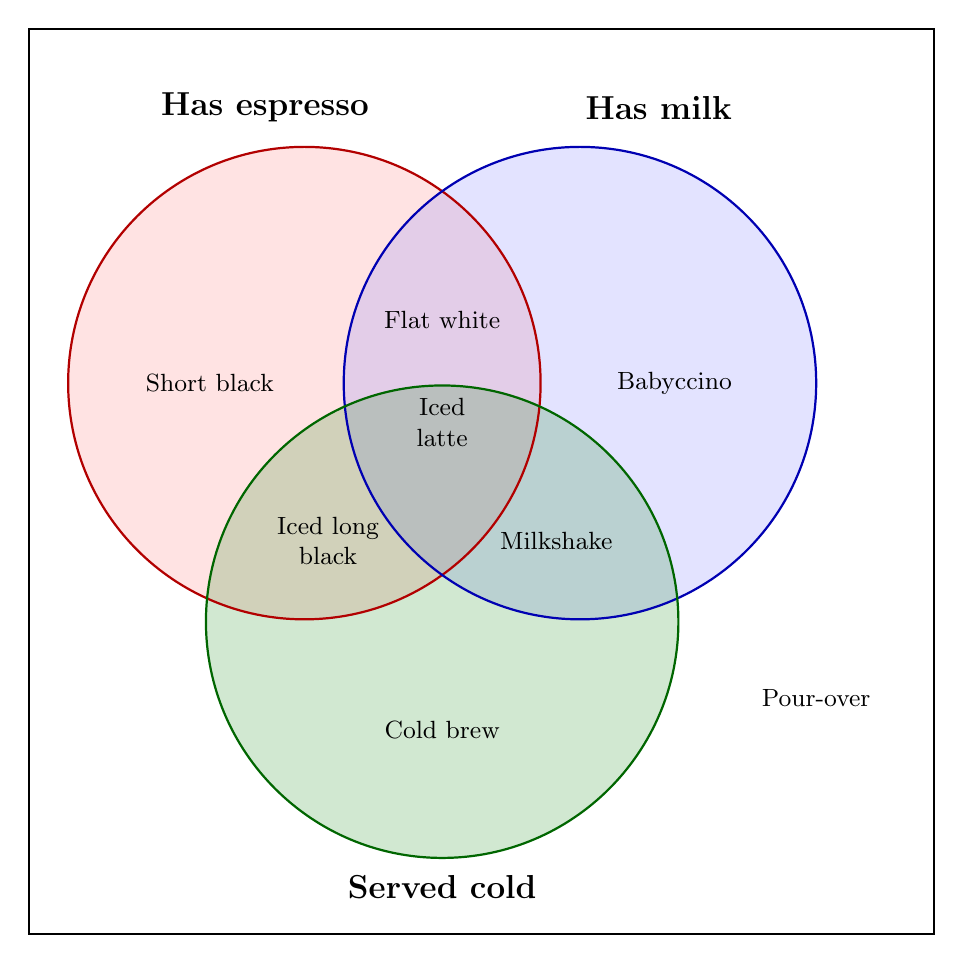
\begin{tikzpicture}[
  every node/.style={font=\small, align=center},
  circ/.style={draw=black, thick, fill opacity=0.18}
]
  % Universal set
  \draw[thick] (-3.5,-7) rectangle (8,4.5);
  \node[anchor=north west, font=\normalsize] at (-3.4,4.4) {};

  % Circles
  \fill[red!60, opacity=0.18] (0,0) circle (3);
  \fill[blue!60, opacity=0.18] (3.5,0) circle (3);
  \fill[green!50!black, opacity=0.18] (1.75,-3.03) circle (3);
  \draw[thick, red!70!black] (0,0) circle (3);
  \draw[thick, blue!70!black] (3.5,0) circle (3);
  \draw[thick, green!40!black] (1.75,-3.03) circle (3);

  % Set labels
  \node[font=\large\bfseries] at (-0.5,3.5) {Has espresso};
  \node[font=\large\bfseries] at (4.5,3.5) {Has milk};
  \node[font=\large\bfseries] at (1.75,-6.4) {Served cold};

  % Drinks by region
  \node at (-1.2,0) {Short black};              % espresso only
  \node at (4.7,0) {Babyccino};                 % milk only
  \node at (1.75,-4.4) {Cold brew};             % cold only
  \node at (1.75,0.8) {Flat white};             % espresso + milk
  \node at (0.3,-2.0) {Iced long\\black};       % espresso + cold
  \node at (3.2,-2.0) {Milkshake};              % milk + cold
  \node at (1.75,-0.5) {Iced\\latte};           % all three
  \node at (6.5,-4.0) {Pour-over};              % none
\end{tikzpicture}
\end{document}
